\section{User Interests}

1. at macro-scope, see user interests on different platforms, and user activity.


fig.b category differences: histogram, x axis: platforms; y axis:
ratio of videos/pv; legend: different categories.

Fig.~\ref{fig:cdf_active_user}, Fig~\ref{fig:ccdf_user_pv},
Fig~\ref{fig:cdf_content_pv}, Fig~\ref{fig:top_video_pv}. 

2. at individual user level, measure user interest dynamics. metrics:
a) entropy; b) pageview of top x (1~3) categories of videos.

fig a : distribution of entropy;
fig b: distribution of top x categories;


In this section, we study the problem of content consistence from the
angle of users. Specifically, we aim to evaluate if users have focused
interests and preferences at both macroscope and individual level. 
\begin{figure*}[t]
\begin{minipage}{0.32\textwidth}
 \centering
	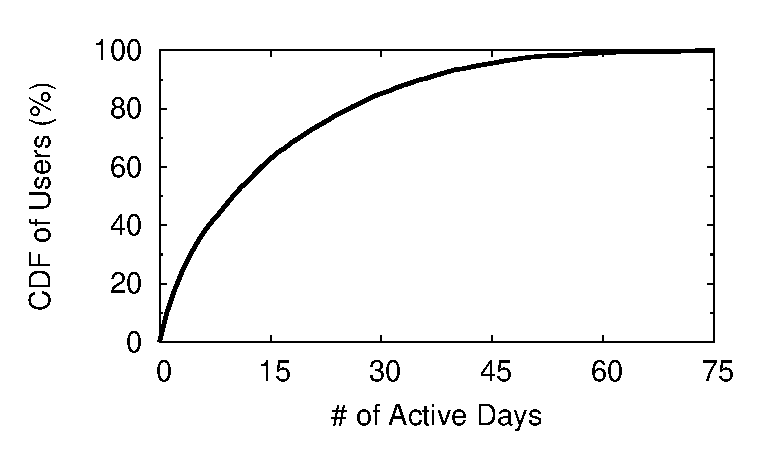
\includegraphics[width=1\textwidth]{plots/basic/cdf_user_active_days.eps}
	\caption{Distribution of user active days.}
	\label{fig:cdf_active_user}
\end{minipage}
\hfill
\begin{minipage}{0.32\textwidth}
 \centering
	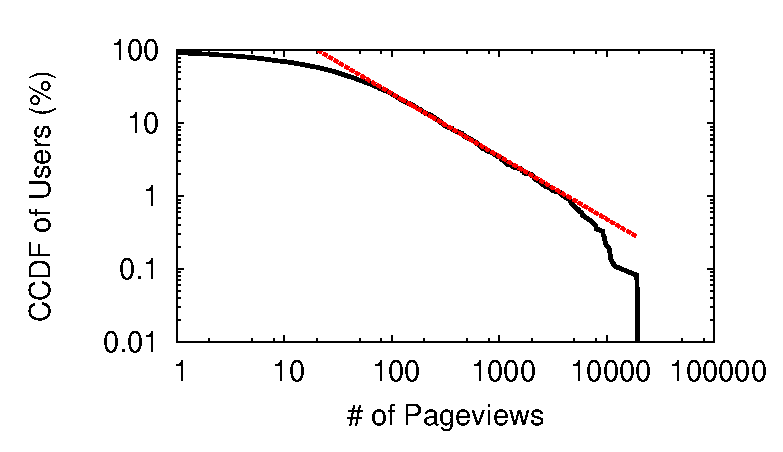
\includegraphics[width=1\textwidth]{plots/basic/ccdf_user_pageviews.eps}
	\caption{Distribution of user pageviews.}
	\label{fig:ccdf_user_pv}
\end{minipage}
\hfill
\begin{minipage}{0.32\textwidth}
 \centering
	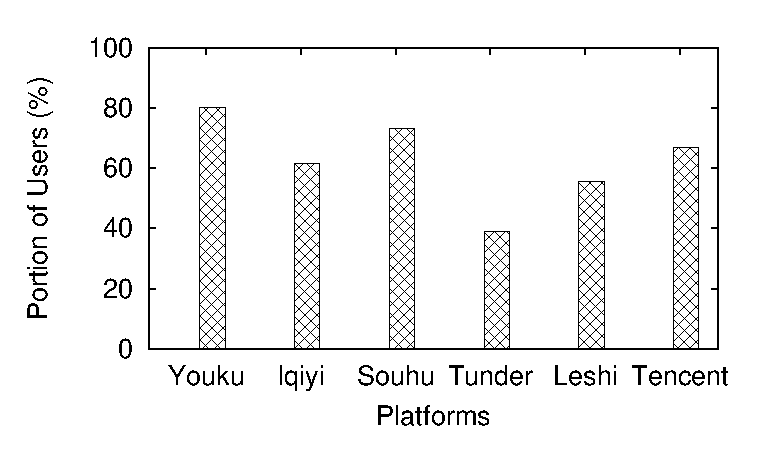
\includegraphics[width=1\textwidth]{plots/users/hist_platform_user.eps}
	\caption{Platform popularity.}
	\label{fig:hist_platform_user}
\end{minipage}
\end{figure*}

\begin{figure*}[t]
\begin{minipage}{0.32\textwidth}
 \centering
	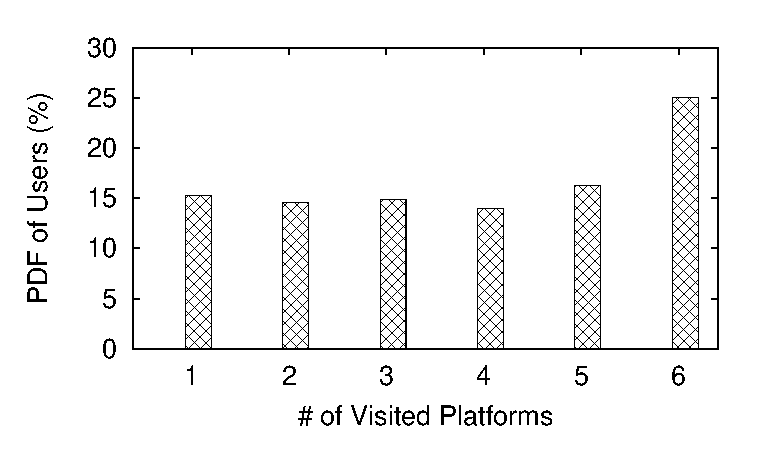
\includegraphics[width=1\textwidth]{plots/users/hist_user_platform.eps}
	\caption{Visited platforms for users.}
	\label{fig:hist_user_platform}
\end{minipage}
\hfill
\begin{minipage}{0.32\textwidth}
 \centering
	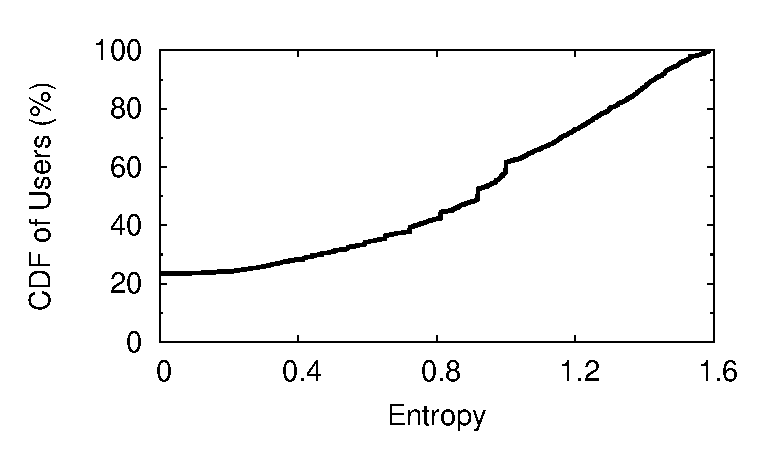
\includegraphics[width=1\textwidth]{plots/users/cdf_entropy.eps}
	\caption{Entropy distribution of user interests.}
	\label{fig:cdf_entropy}
\end{minipage}
\hfill
\begin{minipage}{0.32\textwidth}
 \centering
	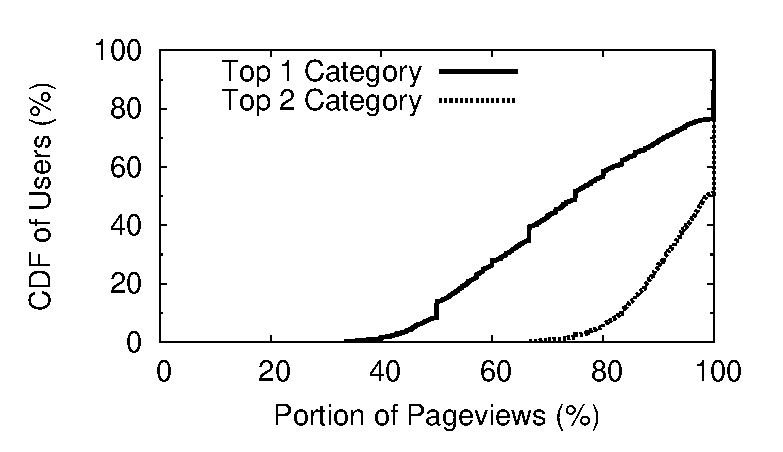
\includegraphics[width=1\textwidth]{plots/users/cdf_top.eps}
	\caption{User interests over categories.}
	\label{fig:cdf_top}
\end{minipage}
\end{figure*}

\subsection{A Macroscope View}

We first investigate user interests and their behavior at macroscope
level. In Fig.~\ref{fig:cdf_active_user}, we plot the distribution of
user active days. For over 50\% users, the number of active days is
more than 10 days. Note that our observation period is about 70
days. That means most users will watch videos at least once per
week. Meanwhile, 20\% users watch videos on at least 30 days. These
super active users watch videos every two days.

We also plot the distribution of pageviews of users in
Figure~\ref{fig:ccdf_user_pv}. As many existing works suggest, a lot
of real world phenomena can be explained by a power-law
distribution~\cite{xxx}. We fit the distribution with a power-law
function ($P(k) \propto k^{-\alpha}$),with a parameter $\alpha=0.86$
and RMSE of $0.001$. This is with our
expectation that a few top users will contribute to most pageviews. 

We then measure users' interests on platforms. In all we have records
of six major video providers in China. Users can visit one or some of
these platforms during our observation period. In
Fig.~\ref{fig:hist_platform_user} we plot the coverage of users for
each platform in our data set. It reveals that users have general
interests on most platforms. The most popular platform, Youku, can
cover around 80\% users. Even the least popular platform, Tunder, can
cover over 40\% users. In Fig.~\ref{fig:hist_user_platform}, we also plot
the number of platforms that users ever visited. Consistent with what
we observe in Fig.~\ref{fig:hist_platform_user}, more than half of
users will visit at least 4 of the 6 platforms. Around 25\% users even
visit all six platforms. 

We then take a look at users' interests on different types of
videos. \fixme{no data here yet.} 

\subsection{An Individual View}
Next, we study user interests from an individual view. We want to
measure if each user has focused interests on several topics. 

To
quantify how a user's interests are focused, we introduce two
metrics. The first metric is entropy~\cite{xxx}. It is defined as the
following formula:
\begin{equation}
H=-\sum p_{i}log(p_{i})
\end{equation}

Here, $H$ is the entropy, and $p_i$ is the probability that a watched
video is of type $i$.  Entropy is an essential metric in information
theory, and it quantifies the information of a probability
distribution. In our work, if a user only watches a single type of
videos, the entropy would be 0. The more focused interests a user has,
the smaller the entropy. In Fig~\ref{fig:cdf_entropy}, we plot the
distribution of entropy of the users. We find more than 20\% of the
users only watch one type of videos. More than half of the users have
an entropy less than 1. 

The other metric quantifies the portion of top types of videos by an
user. Formally, we define it with the following metric:
\begin{equation}
T(k)=\sum_{i<k} P_{i}
\end{equation}

Here $T(k)$ is the metric we  define, and $P_{i}$ is sorted from the
largest one to the least one. $T(k)$ calculates the portion of videos
of top k types. In Fig.~\ref{fig:cdf_top}, we plot this metric when k
equals 1 and 2. 

\fixme{In a more strict case, we evaluate how likely a user will watch the
series of }


The results reveal that users tend to have focused interests on the
videos they watch. In this case, a user is likely to watch videos of
same type as he watched before. This observation provide insights to
predict what video a user will watch in the future.

